\chapter{Analysis}

This section analyses the initial problem described in the introduction. The analysis methods used originates from \cite{mathiassen2001objektorienteret}. 

\section{Introduction}
This chapter aims to provide insight in the system of which this project is based around. The sections and structure of the chapter originates from~\citetitle{mathiassen2001objektorienteret} and includes some of the techniques from~\citetitle{benyon2013designing}. Some general concepts in the system are sought to be derived from the state of the art and how these concepts affects the system is explored further. Based on concepts described in \cref{StateOfTheArt}, a paper prototype of a mobile application is presented in \cref{paperPrototypeSystemChoice}. Conclusively, a specific system definition defines the system of which this project will revolve around.


\section{Problem Statement}
\begin{center}
\textit{How is it possible to develop a software solution which provides a venue with the ability to fairly and dynamically cater to their guests' music preferences?}
\end{center}

Furthermore, the system should take some subproblems into account:
\begin{itemize}
\item How can the system provide supervision and control to the administrators?
\item How can the system avoid undesirable music flow?
\end{itemize}

\section{Interviews}
\label{interviews}

Understanding the people involved in the system is key when doing an analysis, to find their requirements and needs of the system. It is important to get an understanding of current workflows and problems associated with these. One technique towards gaining an understanding of the users, is by interviews. The following section describes how the interviews were conducted and the results that were collected.

\subsection{Procedure}
\label{sub:procedure}
Interviews can be structured, unstructured or anything in between~\cite{benyon2013designing}. Structured interviews are very strict in their form. Every question is pre-made and the interviewer follows the questions strictly. This reduces the effort needed by the interviewer and allows the questions to be well organised and better planned. However this type of interviews should only be used when the answers given by the interviewee are simple and can fall into discrete categories.

On the other end, unstructured interviews allow for a high degree of flexibility. This form of interview is good when knowledge in a particular field is not easily accessible. This flexibility comes with the need for the interviewer to be able to generate questions on the fly and the possibility that these questions are not planned as well and possibly do not cover all aspects.

The interviews described in this section are all semi-structured i.e. most questions are written beforehand but the interviewer is not strictly bound to these and can therefore drill into particular answers given, by following up with related improvised questions. Hence the semi-structured nature of the interviews.

\subsection{Data Collection}
\label{sub:data_collection}
During the interviews the participants were voice recorded and a designated interview helper was taking notes and managing the voice recordings.

\subsection{Interview Analysis}
\label{sub:interview_analysis}
After all the interviews were performed, the group collaboratively created a summary of the interviews, in note-form, by reviewing the voice recordings. Based on the unstructured note-form summary, a more structured summary was made by categorising the notes into key topics. With the more structured interview data, the differences and similarities of the answers given by the participants are now easily extractable. The refined interview data follow each section.

\subsection{Participants}
An important choice in interviewing is who to speak with. There exists two types of people in the interaction this project works with; the bar manager or bartender, who administrates services and protects the interests of the bar, and the guests who visit the bar. The first round of interviews conducted was focused on the administers and can be found in \cref{sub:administersinterviews}. The second round was conducted with the guests at the venue and can be found in \cref{userInterviews}.

\section{Interviews with Administrators}
\label{sub:administersinterviews}
The questions for the administrators were based in the following categories:

\begin{itemize}
  \item Management of bar music systems
  \item Handling requests from the guests
  \item Current and former music systems
  \item Music requirements and the dynamics thereof
\end{itemize}

The full interview guide can be found in \cref{app:interview_guide}.

As this report focuses on the context of bars, the participants would have to have experience working at a bar and using the current music system at the bar. Therefore the sensible choice is to find participants in bars. There are different types of bars: sports bars, bars with DJs at night and bars with a pub atmosphere.

It was chosen to conduct interview with four bars, to get a good representative view of most bars.

\subsection{Control}
\label{sub:Control}
Bars use music to create their image, and music can often be the deciding factor when people are deciding to stay or leave. Therefore all bars expressed, that they want to be in full control of the music, and have the ability to override any request and rearrange the playlist if they feel the need to.

\subsection{Music Flow}
\label{sub:MusicFlow}

All bars want to be able to control the flow of the music. For instance, they do not want a slow track playing right after a party hit in the middle of a party night. This is currently managed by prepopulating a playlist from which the music system plays tracks. Guests can at any time request a track to be played, but no guarantees are given whether the requested track is played or not. When a request is given, the bartender must be the judge of whether or not the requested track is matching the current music theme.

\subsection{Music Systems and DJ}
\label{sub:differences}
Two of the bars have no DJ employed so their music system is in use throughout their opening hours, while the two others have a dedicated DJ playing at night. One participant uses MiB Pro\footnote{\url{http://www.beatpro.dk/mib-bag-baren}}, while the others use Spotify\footnote{\url{https://www.spotify.com/dk/}}. A remark was made that MiB Pro did not have as large a selection of tracks as could be desired.

\subsection{Concerns with stability}
\label{sub:specific_remarks}

One bar owner is concerned with streaming music from the internet, because of potential internet failures. A backup solution working offline would be ideal.

\subsection{Summary}
\label{sub:summary}

From these interviews, requirements have been gathered based on the participants' responses. These requirements are listed beneath using the MoSCoW method introduced in~\cite{benyon2013designing}. This method provides a structured way of prioritising user requirements. It is important to prioritise all requirements because projects do not have unlimited resources, and because of this have to solve the greatest requirements first.

\subsubsection{Must have}

\begin{itemize}\label{musthave}
        \item Ability for the bar to control what music is being played
        \item The system should always play music, no disruption in playback unless desired
\end{itemize}

\subsubsection{Should have}

\begin{itemize}
        \item Ensured continuity in the tracks that are played
\end{itemize}

\subsubsection{Could have}

\begin{itemize}
        \item The ability to take music flow into account
\end{itemize}

\subsubsection{Want to have}

\begin{itemize}
        \item System works offline
\end{itemize}

\section{DJ interview}
One of the important parts from the interview with the pubs was that continuity in the music was very important. So we wanted to get information on how to structure the night at a public place. A DJ has a lot of experience managing music at different events. Thus an interview with DJ Morten Morville was conducted~\cite{int_dj}. The interviews was conducted by members of project group ds320e14 and the result from the interview were shared. Morten is a danish DJ that do gigs at clubs and private parties.

%Some things we got out of the interview with the DJ
The DJ buys music digitally from online music stores like iTunes \footnote{\url{www.apple.com/uk/itunes/}} or beatport \footnote{\url{www.beatport.com/}}. Digital music is easy to carry around, therefore he is able to bring all his music with him all the time. This means he does not have to decide want music to bring ahead of an event.

When building the structure of a night the DJ usually starts with uncommercial music and then later at prime time he will play more mainstream music. At the end of a nigh he likes playing music that can get people going even more.

When playing at club he is more strict with wishes since he is responsible for keeping the music consistent and keeping everyone happy. At private parties he has to be open to wishes.

He is not interested in software to assist him in choosing music or recording the playlist for a night and given feedback.

\subsection{Spotify}
\label{sub:spotify}
Spotify was chosen as the service from which the system would acquire its music data. This was done because a majority of the bars that were interviewed in \cref{interviews}, uses spotify for controlling their music during daytime. Spotify is also a well-established service for streaming music with over 20 million songs.

Spotify provides a API that allows the programmer to develop applications that can access and manage data from spotify’s servers. This means the project group does not have to deal with licensing and a hosting of music data for the system.

Spotify also provides a business plan that allows for playing music to the public. Spotify Business is only available in Sweden right now~\cite{spotifyBusiness}.

\frnote{ret for stavefejl}
\subsection{Persona}
\frnote{ret}
The people that use a system can be represented by personas. This is done in order to ensure the PACT elements are centered in the design process\kanote{Hvad menes der her?}. Personas are general profiles of different types of users. A persona is a concrete representation of a fictitious person. Personas help the designer by having a specific end user in mind, preventing them designing the system for themselves. Personas are developed through the understanding process and through undertaking a PACT analysis. A part of the persona is a short story of the person trying to achieve a goal using the system in a specific context~\cite{benyon2013designing}.

As part of this project, a persona was made, based on the interviews which were conducted.%\cref{interviewbruger}.
This is Camilla, an average user of the system.

\subsubsection{Camilla}
\begin{figure} [h]
  \centering
  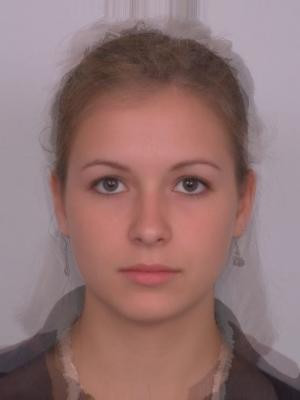
\includegraphics[]{Images/average.jpg}
  \caption{Picture associated with the persona \enquote{Camilla}. Copyright the Face Research Lab. Used with permission.}
  \label{fig:camilla}
\end{figure}
\noindent\textbf{Basic information}
\begin{itemize}
\item 25 years old
\item Medical student
\item Employed in an elderly care center
\item In a relationship with Keith
\item She loves meeting new people
\item When going out she likes to visit small places that allow socialisation
\item Volunteered in Red Cross Uganda
\end{itemize}

It is Friday afternoon and Camilla is planning to meet some of her fellow students at a bar. Camilla and her friends get together after they are finished at school and go to a café to grab a sandwich. After dinner, Camilla takes out her smartphone and checks openPlaylist. Camilla can see that some of her favourite songs are being played at White Hart, and they agree to go there. Upon arriving Camilla checks in via the application. She immediately notices on the screen behind the bar that the queue is filled with songs she dislikes. She now uses the application to request and upvote other songs that she would like to be played. Some other people at White Hart agree on Camilla's choices and they too upvote these songs. On the screen in the bar Camilla can see some of the other people that upvotes her songs and later in the evening she meets them and they talk about all the nice music they have in common. Camilla and her new and old friends party all night long and drink a lot of beer.

\section{State of the Art}
\subsection{SecretDJ}
SecretDJ gives its users the ability to see which venues use the SecretDJ system, and which are nearest to the user. The users can add songs to the venue's playlist and give likes, via Facebook, to the songs, moving them up the playlist.\\

A new user can add four songs to a venue's playlist each day. If a user gets a lot of likes for the songs he has added to a venue's playlist, the user can rise in rank for that venue, which means the user can add more songs to that venue's playlist and that his choices are moved further up the playlist by default. 
If a user gets enough likes and is active enough, the user can rise to the rank of DJ for a venue, meaning that the user's choice of songs will always be next in line, and there is no limit to the amount of songs the user can add to the playlist.


\section{Stakeholders}
\label{interviews}

Understanding the people involved in the system is key when doing an analysis, to find their requirements and needs of the system. It is important to get an understanding of current workflows and problems associated with these. One technique towards gaining an understanding of the users, is by interviews. The following section describes how the interviews were conducted and the results that were collected.

\subsection{Procedure}
\label{sub:procedure}
Interviews can be structured, unstructured or anything in between~\cite{benyon2013designing}. Structured interviews are very strict in their form. Every question is pre-made and the interviewer follows the questions strictly. This reduces the effort needed by the interviewer and allows the questions to be well organised and better planned. However this type of interviews should only be used when the answers given by the interviewee are simple and can fall into discrete categories.

On the other end, unstructured interviews allow for a high degree of flexibility. This form of interview is good when knowledge in a particular field is not easily accessible. This flexibility comes with the need for the interviewer to be able to generate questions on the fly and the possibility that these questions are not planned as well and possibly do not cover all aspects.

The interviews described in this section are all semi-structured i.e. most questions are written beforehand but the interviewer is not strictly bound to these and can therefore drill into particular answers given, by following up with related improvised questions. Hence the semi-structured nature of the interviews.

\subsection{Data Collection}
\label{sub:data_collection}
During the interviews the participants were voice recorded and a designated interview helper was taking notes and managing the voice recordings.

\subsection{Interview Analysis}
\label{sub:interview_analysis}
After all the interviews were performed, the group collaboratively created a summary of the interviews, in note-form, by reviewing the voice recordings. Based on the unstructured note-form summary, a more structured summary was made by categorising the notes into key topics. With the more structured interview data, the differences and similarities of the answers given by the participants are now easily extractable. The refined interview data follow each section.

\subsection{Participants}
An important choice in interviewing is who to speak with. There exists two types of people in the interaction this project works with; the bar manager or bartender, who administrates services and protects the interests of the bar, and the guests who visit the bar. The first round of interviews conducted was focused on the administers and can be found in \cref{sub:administersinterviews}. The second round was conducted with the guests at the venue and can be found in \cref{userInterviews}.

\section{Interviews with Administrators}
\label{sub:administersinterviews}
The questions for the administrators were based in the following categories:

\begin{itemize}
  \item Management of bar music systems
  \item Handling requests from the guests
  \item Current and former music systems
  \item Music requirements and the dynamics thereof
\end{itemize}

The full interview guide can be found in \cref{app:interview_guide}.

As this report focuses on the context of bars, the participants would have to have experience working at a bar and using the current music system at the bar. Therefore the sensible choice is to find participants in bars. There are different types of bars: sports bars, bars with DJs at night and bars with a pub atmosphere.

It was chosen to conduct interview with four bars, to get a good representative view of most bars.

\subsection{Control}
\label{sub:Control}
Bars use music to create their image, and music can often be the deciding factor when people are deciding to stay or leave. Therefore all bars expressed, that they want to be in full control of the music, and have the ability to override any request and rearrange the playlist if they feel the need to.

\subsection{Music Flow}
\label{sub:MusicFlow}

All bars want to be able to control the flow of the music. For instance, they do not want a slow track playing right after a party hit in the middle of a party night. This is currently managed by prepopulating a playlist from which the music system plays tracks. Guests can at any time request a track to be played, but no guarantees are given whether the requested track is played or not. When a request is given, the bartender must be the judge of whether or not the requested track is matching the current music theme.

\subsection{Music Systems and DJ}
\label{sub:differences}
Two of the bars have no DJ employed so their music system is in use throughout their opening hours, while the two others have a dedicated DJ playing at night. One participant uses MiB Pro\footnote{\url{http://www.beatpro.dk/mib-bag-baren}}, while the others use Spotify\footnote{\url{https://www.spotify.com/dk/}}. A remark was made that MiB Pro did not have as large a selection of tracks as could be desired.

\subsection{Concerns with stability}
\label{sub:specific_remarks}

One bar owner is concerned with streaming music from the internet, because of potential internet failures. A backup solution working offline would be ideal.

\subsection{Summary}
\label{sub:summary}

From these interviews, requirements have been gathered based on the participants' responses. These requirements are listed beneath using the MoSCoW method introduced in~\cite{benyon2013designing}. This method provides a structured way of prioritising user requirements. It is important to prioritise all requirements because projects do not have unlimited resources, and because of this have to solve the greatest requirements first.

\subsubsection{Must have}

\begin{itemize}\label{musthave}
        \item Ability for the bar to control what music is being played
        \item The system should always play music, no disruption in playback unless desired
\end{itemize}

\subsubsection{Should have}

\begin{itemize}
        \item Ensured continuity in the tracks that are played
\end{itemize}

\subsubsection{Could have}

\begin{itemize}
        \item The ability to take music flow into account
\end{itemize}

\subsubsection{Want to have}

\begin{itemize}
        \item System works offline
\end{itemize}

\input{Chapters/Analysis/Stakeholders/personas.tex}

\section{Problem and Application Domain}
\sinote{Dette afsnit er design orienteret. Er ikke færdigt}

\textbf{Problem domain}: \enquote{That part of a context that is administrated, monitored or controlled by a system.}

\begin{description}
  \item[Tracks] The tracks that are available for playing.
  % \item[Playlists] Collections of tracks centered around a specific theme.
  \item[Votes] Some mechanism for choosing which tracks to play next.
  \item[Users] Data and statistics of the users of the system.
  \item[Places] What is playing at particular places?
  \item[Audio system] Plays the chosen track.
  \item[Display system] Displays queue, current track, etc. at the installation site.
\end{description}

\textbf{Application domain}: \enquote{The organization that administrates, monitors, or controls a problem domain.}

\begin{description}
  \item[Users] The users of the application chooses which tracks to play next.
  \item[Frontend] Provides control of tracks, playlists and users.
  \item[Backend] Administrates and monitors users of the application. Communicate with the audio- and display system.
\end{description}


\section{System Definition}
%intro til System Description
To concretise the system which is described in this report, this section will present a detailed description of the specification of the system. This section will include a FACTOR analysis, a hallmark of object oriented analysis and design, and a system definition, which will pave the way for the remainder of the report.

\subsection{FACTOR}
FACTOR is a list of criteria that can be use in the process of creating a system definition. This is done by checking the definition against the criterias \cite{mathiassen2001objektorienteret}. A FACTOR were created though the current knowledge of the system. This was done to list and organise the system and domain of where the system should be implemented.
This whas created on the basis of ISMDMUME~\cite{sorensen2012}, adding additional concepts from the rest of the state of the art and combining this with the requirements from both the guests and administrators, found in \cref{sub:administersinterviews} and \cref{userInterviews}, into one system.
\subsubsection{Functionality}
The functionality are what the system should be able. These are mainly formed from the requirements given by both the administrators and guests.
\begin{itemize}
    \item Enable users to submit votes. It was chosen that the best way to cater the guests music preferences fairly and dynamically was though votes. This was done since they enable every user to have the possibility to have the same say in what is to be played while still rewarding more active users, hence fair and equal possibilities for all guests. This also makes it possible to implement dynamic voting since votes and be changed and reset as found fitting.
    \item Administrative overriding of playlist ordering. This was a requirement from the administrators found in \cref{sub:administersinterviews}.
    \item Limit the track space the users can search in, at any given time. A requirement from section \cref{sub:administersinterviews}.
    \item View history of played tracks. A history is modelled in the system to keep track of what has been played. This could be used to keep track of the flow of the music, to ensure music continuity and/or as an extended service for the users.
		\item View the current playlist. The playlist is central for the system, it is what the guests can affect though votes and since it is the order of the tracks what the administrators want to control and make sure follows the venues interests. It is therefore very important to keep track of this and be albe to view.
    \item Playback of tracks.
\end{itemize}

\subsubsection{Application Domain}
The application domain describes what administrators should be able to model in the system. This is found from the interviews with administrators in \cref{sub:administersinterviews}.
\begin{itemize}
    \item Administration of tracks and votes. Remove and restrict tracks.
    \item The order of the tracks on the playlist. They should freely be able to move tracks up and down the playlist as desired.
    \item Playback of the playlist. This includes play, skip track, pause and stop.
\end{itemize}

\subsubsection{Conditions}
The conditions either fount in the interviews or dictated the environment analysed in state of the art.
\begin{itemize}
  \item The client should be minimalistic, so as to improve understandability and learnability, even for intoxicated users
  \item Limitation of what music is allowed at the venue
  \item Has to keep track of which users are on location
\end{itemize}

\subsubsection{Technology}
The technology needed for the system to be fully functional.
\begin{itemize}
    \item Smartphone - For users to interact with the system
    \item Computer - For playing music and storing the playlist, history and votes
		\item Situated display - For the preview interface
    \item Internet
    \item Digital music library
\end{itemize}

\subsubsection{Objects}
The objects modelled by the system.
Requests are not modelled as a object for itself. A unifying concept of vote and request was derived from the ideas of voting and requesting from \cref{StateOfTheArt}. In this concept, votes and request are the same thing. This is done by perceiving all tracks in the music catalogue of the venue, as being eligible for votes, but only tracks with at least one vote will be put on the playlist. This voids the need for requests, while still keeping the functionality, and simplifying the whole system. For these reasons, the rest of the project will work under this unified concept, and will refer to user requests as votes.
\begin{itemize}
  \item Track
  \item Vote
  \item Guest
  \item Playlist
  \item History
  \item Restriction
  \item Administrator
\end{itemize}

\subsubsection{Responsibility}
The responsebility the system will have in the context of a venue.
\begin{itemize}
  \item User influence on music playback
  \item Administrative control for the venue
\end{itemize}

\subsection{System Definition}\label{sub:systemDefinition}
From the FACTOR the system definition were created, clearly defining the system and to be used in the further analysis of the system.

\begin{center}
\textit{An information system enabling venues to have guests vote for tracks to be played. The system should enable the administrators to override the specific tracks and limit the track space the users can vote for, at any given time. The client should be minimalistic, so as to improve understandability and learnability, even for intoxicated users. The system should display already requested tracks to all customers, as to improve discoverability.
The administrative server has to be able to run on an inexpensive computer, with access to a music catalogue and an internet connection of varying stability. The client application has to be able to run on smartphones with unstable internet access and limited data traffic and battery capacity.}
\end{center}

